\subsubsection{Basic Concepts}
\label{sub:dl_concepts}

Understanding more sophisticated deep learning methods used in later
chapters requires comprehension of the basic concepts behind artificial
neural networks.
This chapter introduces mathematical foundations of both neural network
structure and algorithms.
The notation mostly follows the one from Nielsen~\footcite{Nielsen2015}, but also
adds explanations from Bishop~\footcite{Bishop2006} and Goodfellow et al.~\footcite{Goodfellow2016}.
The first paragraph in this subsection will introduce the major elements
of the neural network training process which will then be described in more
detail in the following paragraphs.

\paragraph{Training process}

Like most machine learning algorithms, neural networks are trained using an iterative process.
In short, the network takes some example from the training data set as an input 
and calculates the respective output via a process called 
\textbf{forward propagation}.
Depending on the size of the data set, it repeats this procedure for more 
examples.
Since this constitutes a supervised learning problem, desired outputs for
each example are known.
These can be used to calculate the prediction error, which is determined by the
\textbf{cost function}.
The assessed error can then be used to calculate updates for the parameters of
the networks which are called \textit{weights}.
This process is known as \textbf{backpropagation}.
The examples which are used during one iteration of the training process are
called a \textit{mini-batch}.
A full run through all examples of the training data set is referred to as an
\textit{epoch}.
The forward and backpropagation algorithms and the cost function are the three
basic elements of an artifical neural network. 
In order to define them in more detail, mathematical notation has first to be
established.

\paragraph{Neural network structure}

\begin{figure}[h]
  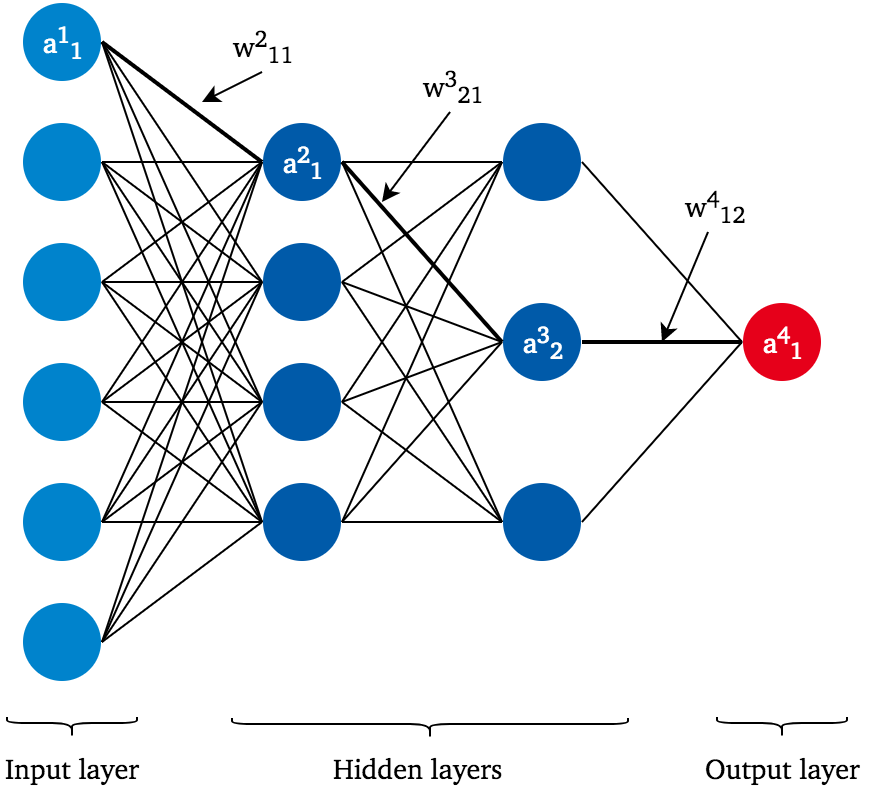
\includegraphics[height=10cm]{img/nn_architecture_2}
  \caption{Neural network structure and notation}
\label{fig:nn_architecture}
\end{figure}

Neural networks basically consist of nodes (also called \textbf{units}) which
are organized as layers.
The single layers of a neural network are wired together via edges that are
called \textbf{weights}.
This subsection will focus on the most basic architecture of a neural network,
called a \textbf{feed-forward network}.
In this architecture all units in a specific layer are connected to all units
in the following layer.
Such a layer is then referred to as being \textit{fully-connected}.
More sophisticated layer architectures will be introduced in subsection~\ref{sub:dl_developments}.
Figure~\ref{fig:nn_architecture} shows an example of a fully-connected network
that contains an input layer with six units, two hidden layers with four respective
three units and and an output layer containing one single unit.
Here, hidden layers are all layers between input and output layer.

In the following, $a_j^l$ will refer to the $j^{th}$ unit in the $l^{th}$ layer.
Weight $w_{jk}^l$ then stands for the weight which connects the $k^{th}$ unit in
the ${(l-1)}^{th}$ layer with the $j^{th}$ unit in the $l^{th}$ layer.
Figure~\ref{fig:nn_architecture} contains an example path from input to ouput
layer which resembles this notation.

\paragraph{Forward propagation}
\label{sub:dl_forward}

During the forward propagation process, the neural network calculates an output
for a specific input with respect to the current weights in the network.
Thus, the network can be written as a function $f(x,w)$ where $x$ is an input
vector or matrix and $w$ is the set of all weights for this network.
The units in the input layer receive their value from the input vector.
All units in later layers are calculated using equation~\ref{eq:activation}.

\begin{equation}
  \label{eq:activation}
  a_j^l = \sigma(\sum_k w_{jk}^l a_k^{l-1} + b_j^l)
\end{equation}

In this equation, $a_j^l$ is also called an \textbf{activation}, $\sigma$ is a
non-linear transformation function and $b_j^l$ is an added bias term.
The bias term is here independent of the activations in the previous layer.
In practice, this calculation can be parallelized for all activations in a layer
by rewriting it in matrix form (see equation~\ref{eq:activation_matrix}).

\begin{equation}
  \label{eq:activation_matrix}
  a^l = \sigma(w^l a^{l-1} + b^l)
\end{equation}

Here, $a^l$ is the vector of all activations in layer $l$, $b^l$ is the vector
of all bias terms in layer $l$ and $a^{l-1}$ is the vector of all activations
in the previous layer. The matrix $w^l$ resembles all connections from layer $(l-1)$
to layer $l$, where $w^l_{jk}$ is the entry in the $j^{th}$ row and $k^{th}$ column.
The function $\sigma$ is applied element-wise to the result vector.

%\outline{What are examples for non-linearities?}
\begin{figure}[h]
  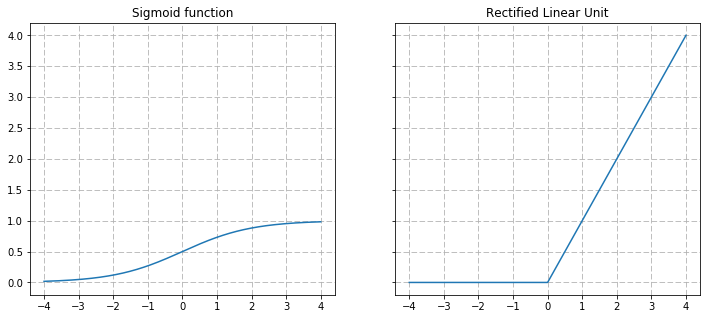
\includegraphics[height=7cm]{img/nn_activations}
  \caption{Popular neural network activation functions}
\label{fig:activations}
\end{figure}

If $\sigma(x) = x$, then the output activations $a^l$ will just be a linear
combination of the input activations $a^{l-1}$.
This property does obviously not change when applied over more layers.
The result will still be a linear function.
In contrast to that, if $\sigma$ is a non-linear function, the network receives more 
representational capability, i.e., it can learn to represent a bigger variety of 
functions. 
Two popular choices for $\sigma$ are the \textit{sigmoid function} and the
\textit{Rectified Linear Unit (ReLU)} (see figure~\ref{fig:activations}). 
The sigmoid function is given by equation~\ref{eq:sigmoid}, whereas ReLU is 
simply equal to the maximum of the input and zero (equation~\ref{eq:relu}).

\begin{equation}
  \label{eq:sigmoid}
  \sigma(x) = \frac{1}{1 + \exp(-x)}
\end{equation}

\begin{equation}
  \label{eq:relu}
  \sigma(x) = \max(0, x)
\end{equation}

Outputs of the sigmoid function are guaranteed to be between zero and one, which fits
the problem of predicting class probabilities.
Hence, the sigmoid function is most commonly applied in output layers of networks that
train on a classification task.
Contrary, most hidden layers in modern neural networks use ReLU as an activation
function.
The function was introduced in 2000 and has shown to be suitable for most deep
learning techniques, since it stabilizes the training process~\footcite{Hahnioser2000, Nair2010}.

All in all, forward propagation is the layer-wise application of above described
calculations. For the example network in figure~\ref{fig:nn_architecture}, the
output for an example data point $x$ can be determined according to equation~\ref{eq:forward_prop}.
The enumerator in $\sigma$ indicates that different activation functions can
be applied in each layer.

\begin{equation}
  \label{eq:forward_prop}
  a^4 = \sigma^4(w^4 \sigma^3(w^3 \sigma^2(w^2 x + b^2) + b^3) + b^4)
\end{equation}

With the calculated outputs it is possible to evaluate predictions of the
networks by calculating the error according to the cost function.

\paragraph{Cost function}

In order to state necessary assumptions about the cost function, a first look
at the goal of the backpropagation algorithm is useful.
Backpropagation aims at deriving updates for all weights and biases in
the network.
It does so by calculating the gradients $\partial C / \partial w$ and 
$\partial C / \partial b$ of the cost function with respect to weights and
biases.
Two assumptions about the cost function have to be made, so that the 
backpropagation algorithm is able to work. 
The reasons for these assumptions will be explained in the next paragraph.
For illustration purposes this paragraph will use the \textit{quadratic cost function}
as a running example (see equation~\ref{eq:quad_costs}).
Here, $y(x)$ is the desired output for input $x$, $n$ resembles the number of
examples in the current mini-batch and $L$ denotes the output layer of the
network.

\begin{equation}
  \label{eq:quad_costs}
  C = \frac{1}{2n} \sum_x \Vert y(x) - a^L(x) \Vert^2
\end{equation}

The first assumption (equation~\ref{eq:cost_assump_1}) is that the cost function 
can be calculated as the average of all error terms for the current batch
of training examples. For example the quadratic cost function can be written in
this form, because $C_x = \frac{1}{2} \Vert y - a^L \Vert^2$.

\begin{equation}
  \label{eq:cost_assump_1}
  C = \frac{1}{n} \sum_x C_x
\end{equation}

Secondly, the cost function has to be a function of the network output $a^L(x)$
(see equation~\ref{eq:cost_assump_2}).
Obviously, this is given for the quadratic cost function since $a^L(x)$ is used
for determining the error and all other components are fixed parameters.

\begin{equation}
  \label{eq:cost_assump_2}
  C = C(a^L)
\end{equation}

With these assumptions set the next paragraph will explain how the
backpropagation algorithm derives gradients for the weight updates which enable
learning in the training process.

\paragraph{Backpropagation}
\label{sub:backprop}

As mentioned before, the backpropagation offers a way to calculate gradients
of the cost function with regard to weights and biases of the network.
Optimization algorithms such as gradient descent then make use of these 
gradients when determining weight updates since they intuitively represent
the rate of change of the cost function with respect to these learnable weights.
This paragraph will explain how the backpropagation algorithm works in detail.
Proofs are out of scope for this thesis and therefore omitted completely.

Some definitions are helpful for the further explanations. Firstly
$z^l$ is defined as an intermediate quantity which represents the weighted
inputs for neurons in layer $l$ (see equation~\ref{eq:weighted_input}).

\begin{equation}
  \label{eq:weighted_input}
  z^l \equiv w^l a^{l-1} + b^l \Rightarrow a^l = \sigma(z^l)
\end{equation}

Another useful intermediate quantity is $\delta_j^l$ which denotes the error
in the $j^{th}$ neuron in the $l^{th}$ layer. The error is defined in
equation~\ref{eq:neuron_error} as the partial gradient of the cost function
with respect to the weighted input to the neuron. Intuitively, if this value
is large (positively or negatively), the cost can be lowered by updating the 
weighted input in the opposite direction.

\begin{equation}
  \label{eq:neuron_error}
  \delta_j^l \equiv \frac{\partial C}{\partial z_j^l}
\end{equation}

The following explanation of the backpropagation algorithm is centered around
the four fundamental equations mentioned by Nielsen~\footcite{Nielsen2015}.
Since the value of the cost function is known after the forward propagation
procedure, the first step of backpropagation is to calculate the error in the
output layer $L$.
Equation~\ref{eq:bp_1_comp} states how this is achieved for a single neuron,
whereas equation~\ref{eq:bp_1_mat} shows the matrix-based form for efficient
computation in practice. In this equation $\nabla_a C$ is the vector of all partial
derivatives $\partial C / \partial a_j^L$ and $\odot$ denotes the element-wise
multiplication of two vectors, known as the \textit{Hadamard product}.
For the previously introduced quadratic cost function, it would simply hold
that $\nabla_a C = (a^L -y)$.
This is also where the assumption about the cost function as a function of the
output activations $a^L$ comes into play.

\begin{equation}
  \label{eq:bp_1_comp}
  \delta_j^L = \frac{\partial C}{\partial a_j^L} \sigma'(z_j^L)
\end{equation}

\begin{equation}
  \label{eq:bp_1_mat}
  \delta^L = \nabla_a C \odot \sigma'(z^L)
\end{equation}

The expresssions can be split into two components. On the one hand, the partial
derivative represents the rate of change of the cost function with respect to
the output activations, on the other hand $\sigma'(z^L)$ determines how
fast the activation function changes for the weighted input.

After the error in the output layer is calculated, the next logical step is to
compute error terms for the previous layers.
In order to do that, the backpropagation algorithm only requires the error in
the next layer (see equation~\ref{eq:bp_2}).

\begin{equation}
  \label{eq:bp_2}
  \delta^l = ({(w^{l+1})}^T \delta^{l+1}) \odot \sigma'(z^l)
\end{equation}

The basic intuition behind this equation is that the known error $\delta^{l+1}$
flows backward through the network by multiplying it with the weight
matrix $w^{l+1}$.
It is then further moved through the activations of neurons in layer $l$ by
building the Hadamard product with the derivative of the activation function.
In summary, the first two equations offer a way to determine the errors for all
layers in the network.
The final two steps now aim to relate the errors to the partial derivatives
$\partial C / \partial w$ and $\partial C / \partial b$.

Equation~\ref{eq:bp_3} shows that the gradient of the cost function with respect
to any bias in the network is equal to the error at that neuron.
In short, this is also written as stated in equation~\ref{eq:bp_3_short}.

\begin{equation}
  \label{eq:bp_3}
  \frac{\partial C}{\partial b_j^l} = \delta_j^l
\end{equation}

\begin{equation}
  \label{eq:bp_3_short}
  \frac{\partial C}{\partial b} = \delta
\end{equation}

For weights, this computation is slightly more complex because they represent
a connection between two neurons.
In order to derive the gradient for a weight, the error in the current layer
has to be multiplied by the activation of the connected neuron in the previous
layer (see equation~\ref{eq:bp_4}).
This implies that weight updates are smaller if the input activation is near
zero.
Hence, the weight is said to \textit{learn slowly}.

\begin{equation}
  \label{eq:bp_4}
  \frac{\partial C}{\partial w_{jk}^l} = a_k^{l-1} \delta_j^l
\end{equation}

Optimization algorithms make use of the computed gradients in that they determine
updates for all weights and biases in the network.
Figure~\ref{fig:grad_desc} illustrates mechanics of most optimization
algorithms used in neural networks.
Here, a common practice is to use mini-batches, i.e., small collections of
examples, for each iteration of the algorithm.
For each example the output of the network is calculated, which is then used
to determine the output error. 
The error in the output layer is then propagated through the network in order
to compute the gradients for weights and biases.
In the final step of the iteration, the weights (including biases) are updated
according to the gradients.
The most basic optimization algorithm called \textbf{gradient descent} uses the
update formula in equations~\ref{eq:gd_update_weights} and~\ref{eq:gd_update_biases}.

\begin{equation}
  \label{eq:gd_update_weights}
  w^l \rightarrow w^l - \frac{\eta}{m} \sum_x \delta^{x,l}{(a^{x,l-1})}^T
\end{equation}

\begin{equation}
  \label{eq:gd_update_biases}
  b^l \rightarrow b^l - \frac{\eta}{m} \sum_x \delta^{x,l}
\end{equation}

It averages over the gradients determined by looking at single examples, which
is only possible through the first assumption about the cost function (see equation~\ref{eq:cost_assump_1}).
Here, $m$ is the number of examples in the batch and $\eta$ resembles the
\textit{learning rate} which is a hyperparameter that has to be set prior to
learning.

\begin{figure}[h]
  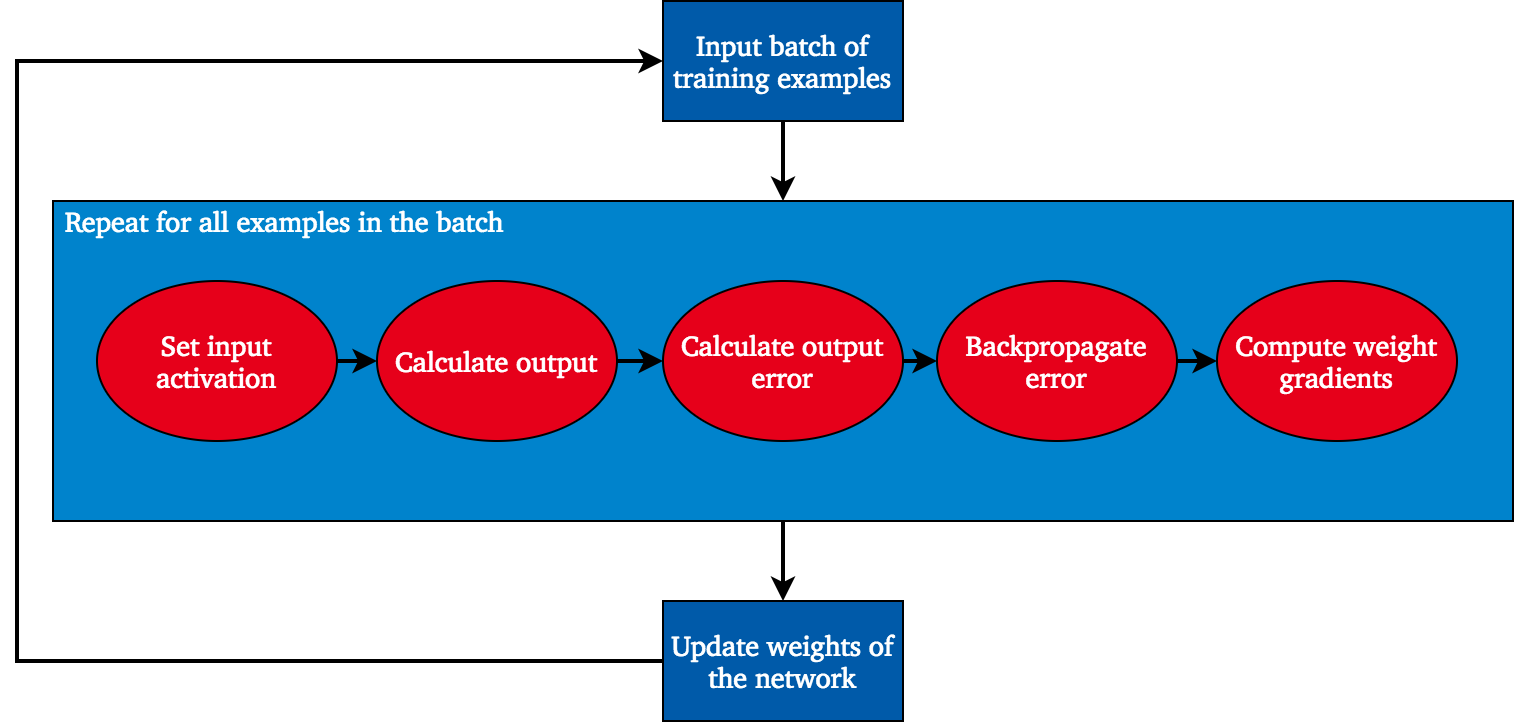
\includegraphics[height=7.5cm]{img/nn_optimization_3}
  \caption{Optimization in neural networks}
\label{fig:grad_desc}
\end{figure}

All in all, the choice of activation function and optimization algorithm largely
influences efficiency and stability of the learning process.
More sophisticated optimization algorithms will be introduced in the next
subsection, along with recent advances regarding architectures and
regularization techniques.
